In \autoref{s:Contribution-2-Motivation} we discuss how ... \hinttext{Explain how this chapter is structured. Make sure you cover all sections!} We summarize our discussion in \autoref{s:Contribution-2-Summary}.

\section{Motivation}
\label{s:Contribution-2-Motivation}

Well... You have to start somewhere. Explain what you did and why. You may assume that the reader already knows the background, related works and major contribution~1.

\section{Major point 1}
\label{s:Contribution-2-Major-1}
Develop your idea! For example, discuss the axioms that underpin the inner workings of your algorithm.

\begin{figure}[h]
\centering
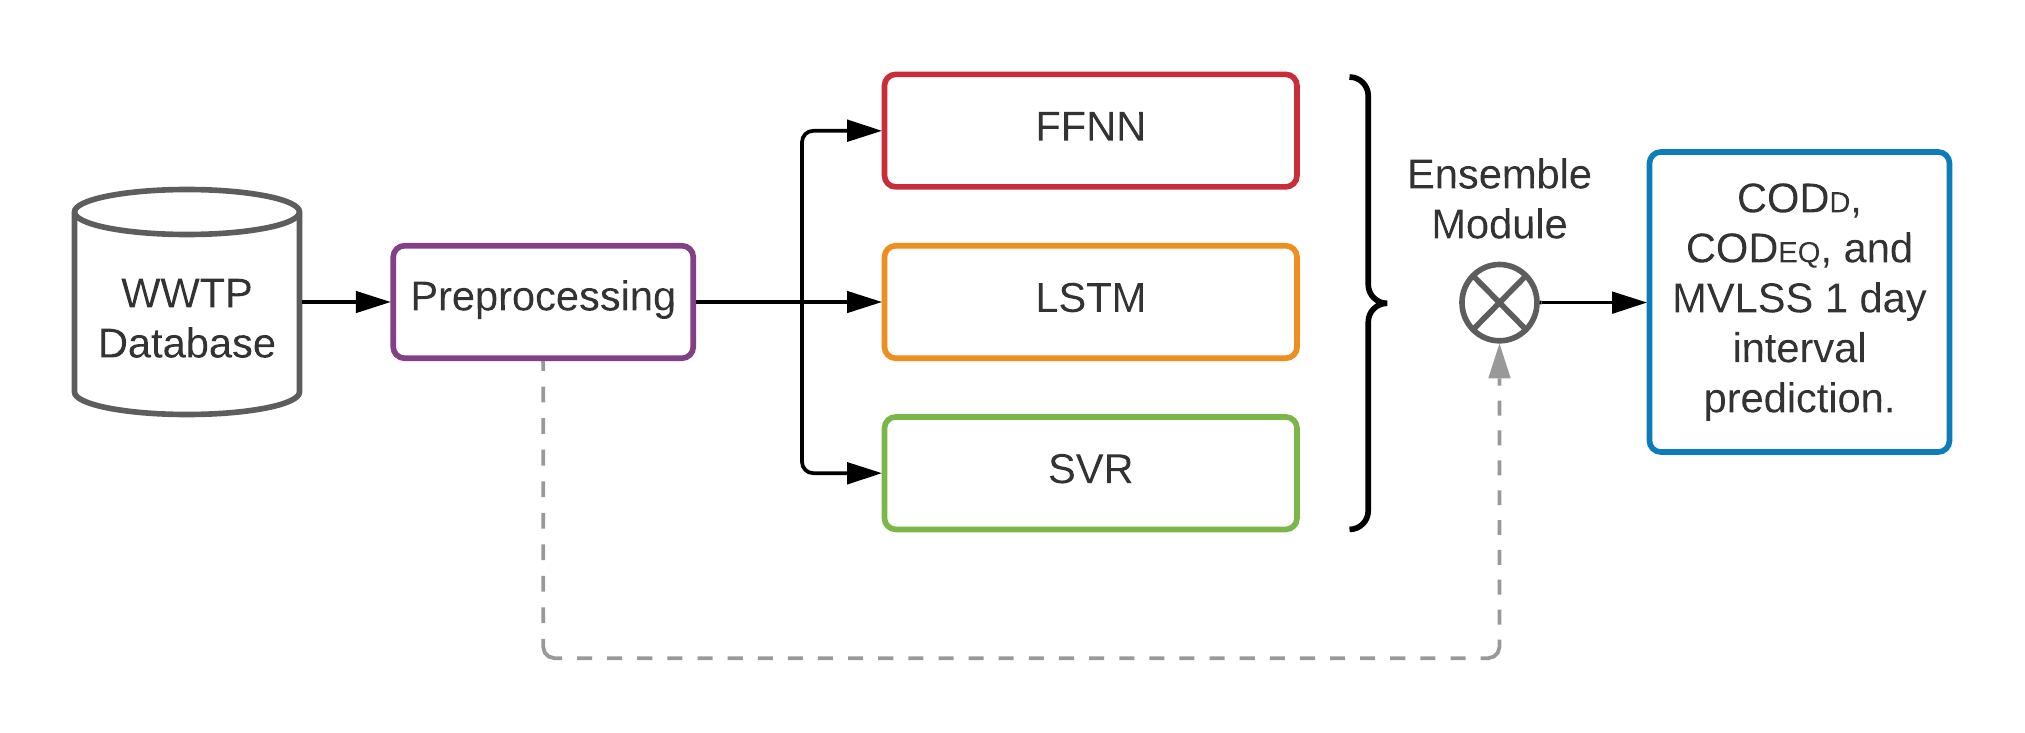
\includegraphics[width=\linewidth]{figures/Ch5/Thesis-Approaches-Ensemble.png}
\caption{Ensemble approach}
\label{f:Ensemble-approach}
\end{figure}


\subsection{Minor idea 1}
\label{s:Contribution-2-Major-1-Minor-1}
Develop your idea! For example, explain how your algorithm actually works.



\subsection{Minor idea 2}
\label{s:Contribution-2-Major-1-Minor-2}
Develop your idea! For example, explain how the theoretical limits of your approach.


\section{Major point 2}
\label{s:Contribution-2-Major-2}
Develop your idea! For example, discuss the difficulties when implementing the proposed algorithm in software.

\subsection{Minor idea 1}
\label{s:Contribution-2-Major-2-Minor-1}
Develop your idea! For example, properties of your implementation.




\subsection{Minor idea 2}
\label{s:Contribution-2-Major-2-Minor-2}
Develop your idea! For example, the particular properties of your implementation.




\section{Summary}
\label{s:Contribution-2-Summary}

Summarize contribution 2. Highlight what makes it relevant. Assuming that the reader knows the details of the contribution now, you should also try to clearly explain in what particular key properties this method deviates from existing research.
